\documentclass{dsa}

\usepackage{shadowtext}
\usepackage{forloop}

\newcommand{\tabularTextInput}[1]{
    \dsaTextInput{#1}{.5\textwidth-4\tabcolsep-2cm}
}

\newcommand{\num}[2][\empty]{
    \ifthenelse{\equal{#1}{\empty}}{
        \raisebox{-0.35ex}{\textField[\ui{align={centered},textsize={12}}]{#2}{1.2cm}{1em}}%
    }{
        \raisebox{-0.35ex}{\textField[\ui{align={centered},textsize={12},bgcolor={#1}}]{#2}{1.2cm}{1.5em}}%
    }%
}
\newcommand{\dsaPropline}[2]{
    \small #1 & \num{#2-modif} & \num{#2-orig} & \cellcolor{white} \num{#2-akt}%
}
\newcommand{\dsaExtProp}[3]{
    \small #1 \hfill \tiny\normalfont\bfseries #2 \hspace{3pt} & \num{#3-modif} & \num{#3-orig} & \cellcolor{white}\num{#3-akt}
}
\newcommand{\dsaExtPropline}[3]{
    \dsaExtProp{#1}{#2}{#3} & \num{#3-bought} & \num{#3-perm}%
}
\newcommand{\smallnum}[1]{
    \hspace{-6pt}\raisebox{-0.35ex}{\textField[\ui{align={centered},textsize={12}}\Ff{\FfReadOnly}]{#1}{0.8cm}{1em}}\hspace{-4pt}%
}
\newcommand{\smalltext}[4][\empty]{%
    \ifthenelse{\equal{#1}{\empty}}{%
        \textField[\textSize{8}\ui{value={\ignorespaces #4}}]{#2}{#3}{10pt}%
    }{%
        \textField[\ui{align={#1},value={\ignorespaces #4}}\textSize{8}]{#2}{#3}{10pt}%
    }%
}
\newcommand{\mediumtext}[3][\empty]{%
    \ifthenelse{\equal{#1}{\empty}}{%
        \raisebox{-0.6ex}{\textField[\textSize{9}]{#2}{#3}{10pt}}%
    }{%
        \raisebox{-0.6ex}{\textField[\ui{align={#1}}\textSize{9}]{#2}{#3}{10pt}}%
    }%
}

\newcommand{\dsaTHeading}[2][1]{\ifthenelse{\equal{#1}{1}}{\centering}{}\raisebox{0.35ex}{\small #2}}

\makeatletter
\newcommand{\roystreqtest}[2]{%
  \ifnum\pdfstrcmp{#1}{#2}=\z@
    \expandafter\@firstoftwo
  \else
    \expandafter\@secondoftwo
  \fi}
\newcommand*{\shifttext}[2]{%
  \settowidth{\@tempdima}{#2}%
  \makebox[\@tempdima]{\hspace*{#1}#2}%
}
\makeatother

\begin{document}

\setlength{\fboxsep}{6pt}

\documentclass{dsa}

\usepackage{shadowtext}
\usepackage{forloop}

\newcommand{\tabularTextInput}[1]{
    \dsaTextInput{#1}{.5\textwidth-4\tabcolsep-2cm}
}

\newcommand{\num}[2][\empty]{
    \ifthenelse{\equal{#1}{\empty}}{
        \raisebox{-0.35ex}{\textField[\ui{align={centered},textsize={12}}]{#2}{1.2cm}{1em}}%
    }{
        \raisebox{-0.35ex}{\textField[\ui{align={centered},textsize={12},bgcolor={#1}}]{#2}{1.2cm}{1.5em}}%
    }%
}
\newcommand{\dsaPropline}[2]{
    \small #1 & \num{#2-modif} & \num{#2-orig} & \cellcolor{white} \num{#2-akt}%
}
\newcommand{\dsaExtProp}[3]{
    \small #1 \hfill \tiny\normalfont\bfseries #2 \hspace{3pt} & \num{#3-modif} & \num{#3-orig} & \cellcolor{white}\num{#3-akt}
}
\newcommand{\dsaExtPropline}[3]{
    \dsaExtProp{#1}{#2}{#3} & \num{#3-bought} & \num{#3-perm}%
}
\newcommand{\smallnum}[1]{
    \hspace{-6pt}\raisebox{-0.35ex}{\textField[\ui{align={centered},textsize={12}}\Ff{\FfReadOnly}]{#1}{0.8cm}{1em}}\hspace{-4pt}%
}
\newcommand{\smalltext}[4][\empty]{%
    \ifthenelse{\equal{#1}{\empty}}{%
        \raisebox{-2pt}{\textField[\textSize{8}\ui{value={\ignorespaces #4}}]{#2}{#3}{11pt}}%
    }{%
        \raisebox{-2pt}{\textField[\ui{align={#1},value={\ignorespaces #4}}\textSize{8}]{#2}{#3}{11pt}}%
    }%
}
\newcommand{\mediumtext}[3][\empty]{%
    \ifthenelse{\equal{#1}{\empty}}{%
        \raisebox{-0.6ex}{\textField[\textSize{9}]{#2}{#3}{13pt}}%
    }{%
        \raisebox{-0.6ex}{\textField[\ui{align={#1}}\textSize{9}]{#2}{#3}{13pt}}%
    }%
}

\newcommand{\dsaTHeading}[2][1]{\ifthenelse{\equal{#1}{1}}{\centering}{}\raisebox{0.35ex}{\small #2}}

\makeatletter
\newcommand{\roystreqtest}[2]{%
  \ifnum\pdfstrcmp{#1}{#2}=\z@
    \expandafter\@firstoftwo
  \else
    \expandafter\@secondoftwo
  \fi}
\newcommand*{\shifttext}[2]{%
  \settowidth{\@tempdima}{#2}%
  \makebox[\@tempdima]{\hspace*{#1}#2}%
}
\makeatother

\setlength{\fboxsep}{6pt}

\newcounter{ct}
\newcounter{cta}
%==============================================================================
% Frontseite: Charaktername & Hintergrund, Vor- und Nachteile, Eigenschaften
%==============================================================================

% Hier lässt sich momentan nichts einstellen.

\newcommand{\tabularTextInput}[1]{%
    \dsaTextInput{#1}{.5\textwidth-4\tabcolsep-2cm}%
}
\tabulinesep=-2pt

\begin{document}

\begin{dsaCharacterSheet}
\setwp{}
\vspace*{10pt}
\renewcommand{\arraystretch}{1.1}
\begin{dsaSheetBox}
    
    \vspace{15pt}
    \begin{center}
        \Huge \shadowtext{Heldendokument}
    \end{center}
    \begin{tabu}{p{2cm}p{\dimexpr.5\textwidth-4\tabcolsep-2cm}p{2cm}p{\dimexpr.5\textwidth-4\tabcolsep-2cm}}
        \textmansontt{Name} & \tabularTextInput{\FroName} & \textmansontt{GP-Basis} & \tabularTextInput{\FroGPBasis} \\ \hline
        \textmansontt{Rasse} & \tabularTextInput{\FroRasse} & \textmansontt{Kultur} & \tabularTextInput{\FroKultur} \\ \hline
        \textmansontt{Profession} & \multicolumn{3}{l}{\dsaTextInput{\FroProfession}{\textwidth-4\tabcolsep-2cm}}
    \end{tabu}
\end{dsaSheetBox}

\vspace{-8pt}
\renewcommand{\tabularTextInput}[1]{
    \dsaTextInput{#1}{\textwidth-3\tabcolsep-2.2cm}
}
\begin{multicols}{2}
\begin{dsaSheetBox}[.5\textwidth-.5\columnsep]
    \begin{tabular}{p{2.2cm}p{\dimexpr\textwidth-4\tabcolsep-2.2cm}}
        \textmansontt{Geschlecht} & \tabularTextInput{\FroGeschlecht} \\ \hline
        \textmansontt{Geburtstag} & \tabularTextInput{\FroGeburtstag} \\ \hline
        \textmansontt{Größe} & \tabularTextInput{\FroGrosse} \\ \hline
        \textmansontt{Gewicht} & \tabularTextInput{\FroGewicht} \\ \hline
        \textmansontt{Haarfarbe} & \tabularTextInput{\FroHaarfarbe} \\ \hline
        \textmansontt{Augenfarbe} & \tabularTextInput{\FroAugenfarbe}
    \end{tabular}
\end{dsaSheetBox}%

\columnbreak%
\begin{dsaSheetBox}[.5\textwidth-.5\columnsep]
    \begin{tabular}{p{2.2cm}p{\dimexpr\textwidth-4\tabcolsep-2.2cm}}
        \textmansontt{Stand} & \tabularTextInput{\FroStand} \\ \hline
        \textmansontt{Sozialstatus} & \tabularTextInput{\FroSozialstatus} \\ \hline
        \textmansontt{Titel} & \tabularTextInput{\FroTitel{0}}%
        \forloop{ct}{1}{\value{ct} < 4}{%
            \\ \hline%
            \multicolumn{2}{p{\dimexpr\textwidth-4\tabcolsep}}{\dsaTextInput{\FroTitel{\thect}}{\textwidth-\tabcolsep}}%
        }%
    \end{tabular}
\end{dsaSheetBox}%
\end{multicols}
\vspace{-12pt}

\begin{dsaSheetBox}[\textwidth]
    \begin{tabular}{p{2.2cm}p{\dimexpr\textwidth-4\tabcolsep-2.2cm}}
        \textmansontt{Aussehen} & \tabularTextInput{\FroAussehen{0}}%
        \forloop{ct}{1}{\value{ct} < 3}{%
            \\ \hline%
            \multicolumn{2}{p{\dimexpr\textwidth-4\tabcolsep}}{\dsaTextInput{\FroAussehen{\thect}}{\textwidth-\tabcolsep}} \\ \hline
        }%
    \end{tabular}
\end{dsaSheetBox}%

\vspace{-8pt}
\begin{multicols}{2}
\begin{center}
    \huge \shadowtext{Vorteile}%
\end{center}%
\vspace{-12pt}%
\begin{dsaSheetBox}[.5\textwidth-.5\columnsep]
    \begin{tabular}{p{\dimexpr\textwidth-2\tabcolsep}}
        \forloop{ct}{0}{\value{ct} < 7}{%
            \ifcase\value{ct}\else\\\hline\fi%
            \dsaTextInput{\FroVorteile{\thect}}{\textwidth-\tabcolsep}%
        }%
    \end{tabular}
\end{dsaSheetBox}

\columnbreak
\begin{center}
    \huge \shadowtext{Nachteile}%
\end{center}%
\vspace{-12pt}%
\begin{dsaSheetBox}[.5\textwidth-.5\columnsep]
    \begin{tabular}{p{\dimexpr\textwidth-2\tabcolsep}}
        \forloop{ct}{0}{\value{ct} < 7}{%
            \ifcase\value{ct}\else\\\hline\fi%
            \dsaTextInput{\FroNachteile{\thect}}{\textwidth-\tabcolsep}%
        }%
    \end{tabular}
\end{dsaSheetBox}
\end{multicols}

\vspace{-32pt}
\begin{center}
    \huge \shadowtext{Eigenschaften \& Basiswerte}
\end{center}

\newcommand{\dsaPropline}[2]{%
    \raisebox{-0.35ex}{\small #1} & \num{\FroEigModifikator{#2}} & \num{\FroEigStartwert{#2}} & \cellcolor{white} \num{\FroEigAktuell{#2}}%
}
\newcommand{\dsaExtProp}[3]{%
    \raisebox{-0.35ex}{\small #1} \hfill \raisebox{-0.35ex}{\tiny\normalfont\bfseries #2} \hspace{3pt} & \num{\FroEigModifikator{#3}} & \num{\FroEigStartwert{#3}} & \cellcolor{white}\num{\FroEigAktuell{#3}}%
}
\newcommand{\dsaExtPropline}[3]{
    \dsaExtProp{#1}{#2}{#3} & \num{\FroEigZugekauft{#3}} & \num{\FroEigPermanent{#3}}%
}

\vspace{-8pt}
\begin{dsaSheetBox}[2\fboxsep + 6.72cm]
    \renewcommand{\arraystretch}{1}
    \setlength{\tabcolsep}{0pt}
    \begin{tabu}{p{3.1cm}|p{1.2cm}|p{1.2cm}!{\vrule width 4\arrayrulewidth}p{1.2cm}}
        \dsaRow{\scriptsize}{\tiny\normalfont\bfseries\centering}{ & Modifikator & Start & Aktuell} \Xhline{2\arrayrulewidth}
        \dsaPropline{Mut}{0} \\ \hline
        \dsaPropline{Klugkeit}{1} \\ \hline
        \dsaPropline{Intuition}{2} \\ \hline
        \dsaPropline{Charisma}{3} \\ \hline
        \dsaPropline{Fingerfertigkeit}{4} \\ \hline
        \dsaPropline{Gewandtheit}{5} \\ \hline
        \dsaPropline{Konstitution}{6} \\ \hline
        \dsaPropline{Körperkraft}{7} \\ \Xhline{2\arrayrulewidth}
        \dsaPropline{Geschwindigkeit}{8}
   \end{tabu}%
\end{dsaSheetBox}
\begin{dsaSheetBox}[2\fboxsep + 11.2cm]
    \renewcommand{\arraystretch}{1}
    \setlength{\tabcolsep}{0pt}
    \begin{tabu}{p{5.1cm}|p{1.2cm}|p{1.2cm}!{\vrule width 4\arrayrulewidth}p{1.2cm}!{\vrule width 4\arrayrulewidth}p{1.2cm}|p{1.2cm}}
        \dsaRow{\scriptsize}{\tiny\normalfont\bfseries\centering}{ & Modifikator & Start & Aktuell & Zugekauft & Permanent} \Xhline{2\arrayrulewidth}
        \dsaExtPropline{Lebenspunkte}{(KO+KO+KK)/2}{9} \\ \hline
        \dsaExtPropline{Ausdauer}{(MU+KO+GE)/2}{10} \\ \hline
        \dsaExtPropline{Astralenergie}{(MU+IN+CH)/2}{11} \\ \hline
        \dsaExtPropline{Karmaenergie}{}{12} \\ \hline
        \dsaExtPropline{Magieresistenz}{(MU+KL+KO)/5}{13} \\ \hline
        \dsaExtProp{INI-Basiswert}{(MU+MU+IN+GE)/5}{14} & \multicolumn{2}{l}{
            \hspace{3pt}\begin{minipage}{2.175cm}\tiny\normalfont
                \vspace{2pt}
                \checkBox[\ui{bgcolor={1 1 1}}\symbolchoice{cross}]{\FroKampfreflexe}{0.13cm}{0.09cm}{on} \raisebox{0.45ex}{Kampfreflexe (INI+4)} \\[1.5pt]
                \checkBox[\ui{bgcolor={1 1 1}}\symbolchoice{cross}]{\FroKampfgespur}{0.13cm}{0.09cm}{on} \raisebox{0.45ex}{Kampfgespür (INI+2)} \hspace{-3pt}
            \end{minipage}
            \vspace{-2pt}
        } \\ \hline
        \dsaExtProp{AT-Basiswert}{(MU+GE+KK)/5}{15} & \multicolumn{2}{c}{\scriptsize \raisebox{-0.45ex}{Wundschwelle}} \\ \cline{1-4}
        \dsaExtProp{PA-Basiswert}{(IN+GE+KK)/5}{16} & \multicolumn{2}{c}{\tiny\normalfont \raisebox{2ex}{(KO/2)+Modifikator}} \\ \cline{1-4}
        \dsaExtProp{FK-Basiswert}{(IN+FF+KK)/5}{17} & \multicolumn{2}{c}{\setlength{\fboxsep}{0pt}\colorbox{white}{\begin{minipage}{1.2cm}\vspace*{2pt}\num{\FroWundschwelle}\end{minipage}}\vspace{-1pt}}
    \end{tabu}
\end{dsaSheetBox}

\vspace{-20pt}
\begin{center}
    \huge \shadowtext{Abenteuerpunkte}
\end{center}
\vspace{-8pt}

\begin{dsaSheetBox}[\textwidth]
    \Large

    \vspace{-5pt}
    \begin{tabular}{p{2cm}p{3cm}p{2.7cm}p{2.5cm}p{2.5cm}p{2.5cm}}
        Gesamt: & \raisebox{-0.45ex}{\textField[\textSize{12}]{\FroAbeGesamt}{2.5cm}{16pt}} & Eingesetzt: & \raisebox{-0.45ex}{\textField[\textSize{12}]{\FroAbeEingesetzt}{2.5cm}{16pt}} & Guthaben: & \raisebox{-0.45ex}{\textField[\textSize{12}]{\FroAbeGuthaben}{2.5cm}{16pt}}
    \end{tabular}
    \vspace{-3pt}
\end{dsaSheetBox}

\begin{tikzpicture}[remember picture, overlay]
    \node[inner sep=0pt] at ([xshift=-0.8cm,yshift=-2.4cm]current page.north) {%
        \includegraphics[width=6cm]{fanpaket/logo-fanprodukt.png}%
    };%
\end{tikzpicture}

\end{dsaCharacterSheet}

\end{document}

%==============================================================================
% Sonderfertigkeiten & Talente
%==============================================================================

\begin{dsaCharacterSheet}

\vspace*{4pt}
\begin{dsaSheetBox}[\textwidth]
    \vspace{1pt}
    \begin{tabular}{llllllllllllllllll}
        MU: & \smallnum{MU-akt} & KL: & \smallnum{KL-akt} & IN: & \smallnum{IN-akt} & CH: & \smallnum{CH-akt} & FF: & \smallnum{FF-akt} & GE: & \smallnum{GE-akt} & KO: & \smallnum{KO-akt} & KK: & \smallnum{KK-akt} & BE: & \smallnum{BE}
    \end{tabular}
    \vspace{-1pt}
\end{dsaSheetBox}

\vspace{-16pt}
\begin{center}
    \huge \shadowtext{Sonderfertigkeiten \& Talente}%
\end{center}%
\vspace{-8pt}

\newcounter{ct}
\newcounter{ct2}

\begin{dsaSheetBox}[\textwidth]

    \renewcommand{\arraystretch}{1}
    \setlength{\tabcolsep}{1pt}
    \normalfont\bfseries
    \newcommand{\Sonderfertigkeiten}[1]{
        \raisebox{0.45ex}{\textmansontt{\Large Sonderfertigkeiten (außer Kampf)}}

        \tiny
        \begin{tabular}{p{.5\textwidth-.5\columnsep-.5\fboxsep}} \hline
            \forloop{ct}{0}{\value{ct} < #1}%
            {%
              \smalltext{Sonderfertigkeiten-Allgemein\thect}{.5\textwidth-.5\columnsep-.5\fboxsep}{} \\ \hline
            }
        \end{tabular}
    }
    \newcommand{\Kampftechniken}[1]{
        \tiny
        \ifcase\MSpalte\relax
            \begin{tabular}{p{0.2cm}|p{4.6cm}|p{0.4cm}|p{1cm}|p{0.7cm}!{\footnotesize\raisebox{-0.2pt}{•}}p{0.7cm}|p{0.8cm}}
                \multicolumn{3}{l|}{\Large \raisebox{0.35ex}{\textmansontt{Kampftechniken}}} & \footnotesize\centering BE & \footnotesize\centering AT & \footnotesize\centering PA & \footnotesize\hspace{0.5pt} TaW
                \forloop{ct}{0}{\value{ct} < #1}%
                {%
                    \\ \hline
                    \checkBox[\symbolchoice{star}\BC{}]{Kampftechniken-SE\thect}{0.2cm}{0.2cm} &
                    \smalltext{Kampftechniken-Name\thect}{4.6cm}{\KampftechnikenBasis{\thect}{0}} &
                    \smalltext[centered]{Kampftechniken-Spalte\thect}{0.4cm}{\KampftechnikenBasis{\thect}{1}} &
                    \smalltext[centered]{Kampftechniken-BE\thect}{1cm}{\KampftechnikenBasis{\thect}{2}} &
                    \smalltext[centered]{Kampftechniken-AT\thect}{0.7cm}{} &
                    \smalltext[centered]{Kampftechniken-PA\thect}{0.7cm}{} &
                    \smalltext[centered]{Kampftechniken-TaW\thect}{0.8cm}{}%
                } \\ \hline
            \end{tabular}
        \else
            \begin{tabular}{p{0.2cm}|p{4.15cm}|p{0.4cm}|p{1cm}|p{0.7cm}!{\footnotesize\raisebox{-0.2pt}{•}}p{0.7cm}|p{0.8cm}|p{0.4cm}}
                \multicolumn{3}{l|}{\Large \raisebox{0.35ex}{\textmansontt{Kampftechniken}}} & \footnotesize\centering BE & \footnotesize\centering AT & \footnotesize\centering PA & \footnotesize\hspace{0.5pt} TaW & \footnotesize\hspace{1pt} M
                \forloop{ct}{0}{\value{ct} < #1}%
                {%
                    \\ \hline
                    \checkBox[\symbolchoice{star}\BC{}]{Kampftechniken-SE\thect}{0.2cm}{0.2cm} &
                    \smalltext{Kampftechniken-Name\thect}{4.15cm}{\KampftechnikenBasis{\thect}{0}} &
                    \smalltext[centered]{Kampftechniken-Spalte\thect}{0.4cm}{\KampftechnikenBasis{\thect}{1}} &
                    \smalltext[centered]{Kampftechniken-BE\thect}{1cm}{\KampftechnikenBasis{\thect}{2}} &
                    \smalltext[centered]{Kampftechniken-AT\thect}{0.7cm}{} &
                    \smalltext[centered]{Kampftechniken-PA\thect}{0.7cm}{} &
                    \smalltext[centered]{Kampftechniken-TaW\thect}{0.8cm}{} &
                    \shifttext{-0.1cm}{\smalltext[centered]{Kampftechniken-M\thect}{0.6cm}{}}%
                } \\ \hline
            \end{tabular}
        \fi

        \vspace{8pt}
    }

    \newcommand{\SprachenSchriften}[1]{
        \begin{tabular}{p{0.2cm}|p{6.85cm}|p{1cm}|p{0.8cm}}
            \multicolumn{2}{l|}{\Large \raisebox{0.35ex}{\textmansontt{Sprachen \& Schriften}}} &
            \footnotesize\centering Komp. & \footnotesize\hspace{0.5pt} TaW
            \forloop{ct}{0}{\value{ct} < #1}{%
                \\ \hline
                \checkBox[\symbolchoice{star}\BC{}]{Kampftechniken-SE\thect}{0.2cm}{0.2cm} &
                \ifthenelse{\equal{\thect}{0}}{
                    \normalfont\fontsize{8pt}{1em}\selectfont Muttersprache:
                    \smalltext{Sprachen-Name\thect}{5cm}{\SprachenBasis{\thect}{0}} &
                }{
                    \smalltext{Sprachen-Name\thect}{6.85cm}{\SprachenBasis{\thect}{0}} &
                }
                \smalltext[centered]{Sprachen-Komp\thect}{1cm}{\SprachenBasis{\thect}{1}} &
                \smalltext[centered]{Sprachen-TaW\thect}{0.8cm}{}%
            } \\ \hline
        \end{tabular}

        \vspace{8pt}
    }

    \newcommand{\Talentliste}[7]{% #1=Feldname-Präfix, #2=Anzeigename, #3=Anzahl, #4=Mirakel?, #5=BE?, #6=Voreingestellte Werte, #7=Mögliche Werte
        \tiny
        \ifcase#4\relax
            \ifcase#5\relax
                \begin{tabular}{p{0.2cm}|p{5.8cm}|p{0.5cm}!{\footnotesize\raisebox{-0.6pt}{•}}p{0.5cm}!{\footnotesize\raisebox{-0.6pt}{•}}p{0.5cm}|p{0.8cm}}
                    \multicolumn{5}{l|}{\Large \raisebox{0.35ex}{\textmansontt{#2}}} & \footnotesize\hspace{0.5pt} TaW
                    \forloop{ct}{0}{\value{ct} < #3}{%
                        \\ \hline
                        \checkBox[\symbolchoice{star}\BC{}]{#1-SE\thect}{0.2cm}{0.2cm} &
                        \ifthenelse{\equal{\TalenteInCombo}{1}}{
                            \raisebox{-0.3ex}{\comboBox[\Ff\FfEdit\ui{value={#6{\thect}{0}}}\textSize{8}\W{0}]{#1-Name\thect}{5.8cm}{10pt}{#7}}
                        }{
                            \smalltext{#1-Name\thect}{5.8cm}{#6{\thect}{0}}
                        } &
                        \shifttext{-0.15cm}{\smalltext[centered]{#1-Eigenschaft1-\thect}{0.7cm}{#6{\thect}{1}}} &
                        \shifttext{-0.15cm}{\smalltext[centered]{#1-Eigenschaft2-\thect}{0.7cm}{#6{\thect}{2}}} &
                        \shifttext{-0.15cm}{\smalltext[centered]{#1-Eigenschaft3-\thect}{0.7cm}{#6{\thect}{3}}} &
                        \smalltext[centered]{#1-TaW\thect}{0.8cm}{}%
                    } \\ \hline
                \end{tabular}
            \else
                \begin{tabular}{p{0.2cm}|p{4.7cm}|p{0.5cm}!{\footnotesize\raisebox{-0.6pt}{•}}p{0.5cm}!{\footnotesize\raisebox{-0.6pt}{•}}p{0.5cm}|p{1.0cm}|p{0.8cm}|p{0.4cm}}
                    \multicolumn{5}{l|}{\Large \raisebox{0.35ex}{\textmansontt{#2}}} & \footnotesize\centering BE & \footnotesize\hspace{0.5pt} TaW
                    \forloop{ct}{0}{\value{ct} < #3}{%
                        \\ \hline
                        \checkBox[\symbolchoice{star}\BC{}]{#1-SE\thect}{0.2cm}{0.2cm} &
                        \ifthenelse{\equal{\TalenteInCombo}{1}}{
                            \raisebox{-0.1ex}{\comboBox[\Ff\FfEdit\ui{value={#6{\thect}{0}}}\textSize{8}\W{0}]{#1-Name\thect}{4.7cm}{10pt}{#7}}
                        }{
                            \smalltext{#1-Name\thect}{4.7cm}{#6{\thect}{0}}
                        } &
                        \shifttext{-0.15cm}{\smalltext[centered]{#1-Eigenschaft1-\thect}{0.7cm}{#6{\thect}{1}}} &
                        \shifttext{-0.15cm}{\smalltext[centered]{#1-Eigenschaft2-\thect}{0.7cm}{#6{\thect}{2}}} &
                        \shifttext{-0.15cm}{\smalltext[centered]{#1-Eigenschaft3-\thect}{0.7cm}{#6{\thect}{3}}} &
                        \smalltext[centered]{#1-BE\thect}{1cm}{#6{\thect}{4}} &
                        \smalltext[centered]{#1-TaW\thect}{0.8cm}{}%
                    } \\ \hline
                \end{tabular}
            \fi
        \else
            \ifcase#5
                \begin{tabular}{p{0.2cm}|p{5.4cm}|p{0.5cm}!{\footnotesize\raisebox{-0.6pt}{•}}p{0.5cm}!{\footnotesize\raisebox{-0.6pt}{•}}p{0.5cm}|p{0.8cm}|p{0.4cm}}
                    \multicolumn{5}{l|}{\Large \raisebox{0.35ex}{\textmansontt{#2}}} & \footnotesize\hspace{0.5pt} TaW & \footnotesize\hspace{1pt} M
                    \forloop{ct}{0}{\value{ct} < #3}{%
                        \\ \hline
                        \checkBox[\symbolchoice{star}\BC{}]{#1-SE\thect}{0.2cm}{0.2cm} &
                        \ifthenelse{\equal{\TalenteInCombo}{1}}{
                            \raisebox{-0.3ex}{\comboBox[\Ff\FfEdit\ui{value={#6{\thect}{0}}}\textSize{8}\W{0}]{#1-Name\thect}{5.4cm}{10pt}{#7}}
                        }{
                            \smalltext{#1-Name\thect}{5.4cm}{#6{\thect}{0}}
                        } &
                        \shifttext{-0.15cm}{\smalltext[centered]{#1-Eigenschaft1-\thect}{0.7cm}{#6{\thect}{1}}} &
                        \shifttext{-0.15cm}{\smalltext[centered]{#1-Eigenschaft2-\thect}{0.7cm}{#6{\thect}{2}}} &
                        \shifttext{-0.15cm}{\smalltext[centered]{#1-Eigenschaft3-\thect}{0.7cm}{#6{\thect}{3}}} &
                        \smalltext[centered]{#1-TaW\thect}{0.8cm}{} &
                        \shifttext{-0.1cm}{\smalltext[centered]{#1-M\thect}{0.6cm}{}}%
                    } \\ \hline
                \end{tabular}
            \else
                \begin{tabular}{p{0.2cm}|p{4.3cm}|p{0.5cm}!{\footnotesize\raisebox{-0.6pt}{•}}p{0.5cm}!{\footnotesize\raisebox{-0.6pt}{•}}p{0.5cm}|p{1.0cm}|p{0.8cm}|p{0.4cm}}
                    \multicolumn{5}{l|}{\Large \raisebox{0.35ex}{\textmansontt{#2}}} & \footnotesize\centering BE & \footnotesize\hspace{0.5pt} TaW & \footnotesize\hspace{1pt} M
                    \forloop{ct}{0}{\value{ct} < #3}{%
                        \\ \hline
                        \checkBox[\symbolchoice{star}\BC{}]{#1-SE\thect}{0.2cm}{0.2cm} &
                        \ifthenelse{\equal{\TalenteInCombo}{1}}{
%                        \ChoiceMenu[combo, width=4.3cm, height=10pt, default=#6{\thect}{0}]{#1-Name\thect}{\KoerperTalentliste} &
                            \raisebox{-0.3ex}{\comboBox[\Ff\FfEdit\ui{value={#6{\thect}{0}}}\textSize{8}\W{0}]{#1-Name\thect}{4.3cm}{10pt}{#7}}
                        }{
                            \smalltext{#1-Name\thect}{4.3cm}{#6{\thect}{0}}
                        } &
                        \shifttext{-0.15cm}{\smalltext[centered]{#1-Eigenschaft1-\thect}{0.7cm}{#6{\thect}{1}}} &
                        \shifttext{-0.15cm}{\smalltext[centered]{#1-Eigenschaft2-\thect}{0.7cm}{#6{\thect}{2}}} &
                        \shifttext{-0.15cm}{\smalltext[centered]{#1-Eigenschaft3-\thect}{0.7cm}{#6{\thect}{3}}} &
                        \smalltext[centered]{#1-BE\thect}{1cm}{#6{\thect}{4}} &
                        \smalltext[centered]{#1-TaW\thect}{0.8cm}{} &
                        \shifttext{-0.1cm}{\smalltext[centered]{#1-M\thect}{0.6cm}{}}%
                    } \\ \hline
                \end{tabular}
            \fi
        \fi

        \vspace{8pt}
    }
    \newcommand{\Gaben}[2][Gaben]{\Talentliste{Gaben}{#1}{#2}{0}{0}{\leer}{}}
    \newcommand{\KoerperlicheTalente}[1]{\Talentliste{Koerper}{Körperliche Talente}{#1}{\MSpalte}{1}{\KoerperBasis}{\KoerperTalentliste}}
    \newcommand{\GesellschaftlicheTalente}[1]{\Talentliste{Gesellschaft}{Gesellschaftliche Talente}{#1}{\MSpalte}{0}{\GesellschaftBasis}{\GesellschaftTalentliste}}
    \newcommand{\NaturTalente}[1]{\Talentliste{Natur}{Naturtalente}{#1}{\MSpalte}{0}{\NaturBasis}{\NaturTalentliste}}
    \newcommand{\WissensTalente}[1]{\Talentliste{Wissen}{Wissenstalente}{#1}{\MSpalte}{0}{\WissenBasis}{\WissenTalentliste}}
    \newcommand{\HandwerklicheTalente}[1]{\Talentliste{Handwerk}{Handwerkliche Talente}{#1}{\MSpalte}{0}{\HandwerkBasis}{\HandwerkTalentliste}}

    \newcommand{\kampf}[4]{
        \ifcase#1%
            #2%
        \or #3%
        \or #4%
        \fi%
    }
    \newcommand{\talent}[6]{\ifcase#1#2\or#3\or#4\or#5\or#6\fi}
    \newcommand{\sprache}[3]{
        \ifcase#1%
            #2%
        \or #3%
        \fi%
    }

    \newcommand{\leer}[2]{}

    \newcommand{\MSpalte}{1}
\newcommand{\TalenteInCombo}{0}

\newcommand{\TalenteLinks}{
	\Sonderfertigkeiten{6}
	\Gaben[Übernatürliche Begabungen]{2}
    \Kampftechniken{11}
	\KoerperlicheTalente{17}
	\GesellschaftlicheTalente{10}
}

\newcommand{\TalenteRechts}{
	\vspace*{-11pt}
	\NaturTalente{8}
	\WissensTalente{15}
	\SprachenSchriften{10}
	\vspace{2pt}
	\HandwerklicheTalente{15}
}

\newcommand{\lparen}{(}
\newcommand{\rparen}{)}
\input{talentbogen-extern.tex}
    
    \setlength{\columnseprule}{1pt}
    \setlength{\columnsep}{4pt}
    \begin{multicols}{2}
        \TalenteLinks

    \columnbreak
        \TalenteRechts
    \end{multicols}
\end{dsaSheetBox}

%
\end{dsaCharacterSheet}

%==============================================================================
% Kampfbogen
%==============================================================================

\begin{dsaCharacterSheet}

\renewcommand{\arraystretch}{1}
 \setlength{\tabcolsep}{1pt}

\vspace*{4pt}
\begin{dsaSheetBox}[\textwidth]
    \vspace{1pt}
    \begin{tabular}{llllllll}
        Attacke-Basiswert: & \smallnum{AT-akt} & Parade-Basiswert: & \smallnum{PA-akt} & Fernkampf-Basiswert: & \smallnum{FK-akt} & Initiative-Basiswert: & \smallnum{INI-akt}
    \end{tabular}
    \vspace{-1pt}
\end{dsaSheetBox}

\vspace{-16pt}
\begin{center}
    \huge \shadowtext{Waffen \& Kampfwerte}%
\end{center}%
\vspace{-8pt}

\newcommand{\Nahkampfwaffen}[2]{%
    \begin{dsaSheetBox}[\textwidth]
        \tiny
        \begin{tabu}{p{4.8cm}|p{2.4cm}|p{1cm}|p{1.4cm}|p{1.6cm}|p{1cm}|p{1.4cm}|p{0.8cm}|p{0.8cm}|p{1.4cm}|p{0.5cm}|p{0.5cm}}
        \dsaTHeading[0]{Nahkampfwaffe} &
        \dsaTHeading{Typ/eBE} &
        \dsaTHeading{DK} &
        \dsaTHeading{TP} &
        \dsaTHeading{TP/KK} &
        \dsaTHeading{INI} &
        \dsaTHeading{WM} &
        \dsaTHeading{AT} &
        \dsaTHeading{PA} &
        \dsaTHeading{TP} &
        \multicolumn{2}{c}{\dsaTHeading[0]{BF}}
        \forloop{ct}{0}{\value{ct} < #1}{%
            \ifcase\value{ct}%
                \\ \Xhline{2\arrayrulewidth}
            \else
                \\ \hline
            \fi
            \mediumtext{Nahkampfwaffe-\thect}{4.8cm} &
            \mediumtext[centered]{NK--Typ-eBE-\thect}{2.4cm} &
            \mediumtext[centered]{NK-DK-\thect}{1cm} &
            \mediumtext[centered]{NK-TPbase-\thect}{1.4cm} &
            \mediumtext[centered]{NK-TP-KK-\thect}{1.6cm} &
            \mediumtext[centered]{NK-INI-\thect}{1cm} &
            \mediumtext[centered]{NK-WM-\thect}{1.4cm} &
            \mediumtext[centered]{NK-AT-\thect}{0.8cm} &
            \mediumtext[centered]{NK-PA-\thect}{0.8cm} &
            \mediumtext[centered]{NK-TP-\thect}{1.4cm} &
            \mediumtext[centered]{NK-BFa-\thect}{0.5cm} &
            \mediumtext[centered]{NK-BFb-\thect}{0.5cm}
        } \\ \Xhline{3\arrayrulewidth}
        \end{tabu}

        \vspace{2pt}
        \ifthenelse{\equal{#2}{0}}{}{
            \begin{tabular}{p{4cm}p{\textwidth-\fboxsep-\tabcolsep-4cm}} \dsaTHeading[0]{Sonderfertigkeiten} & \mediumtext{NK-SF-0}{\textwidth-\fboxsep-\tabcolsep-4cm}
                \forloop{ct}{1}{\value{ct} < #2}{%
                    \\ \hline
                    \multicolumn{2}{l}{\mediumtext{NK-SF-\thect}{\textwidth-\fboxsep}}
                } \\ \hline
            \end{tabular}
        }
    \end{dsaSheetBox}
}

\newcommand{\Fernkampfwaffen}[2]{%
    \begin{dsaSheetBox}[\textwidth]
        \tiny
        \begin{tabu}{p{4.8cm}|p{2.4cm}|p{1.4cm}|p{3.2cm}|p{3.2cm}|p{0.8cm}|p{0.5cm}|p{0.5cm}|p{0.5cm}|p{0.5cm}}
            \dsaTHeading[0]{Fernkampfwaffe} &
            \dsaTHeading{Typ/eBE} &
            \dsaTHeading{TP} &
            \dsaTHeading{Entfernungen} &
            \dsaTHeading{TP/Entfernung} &
            \dsaTHeading{FK} &
            \multicolumn{4}{c}{\dsaTHeading[0]{Geschosse}}
            \forloop{ct}{0}{\value{ct} < #1}{%
                \ifcase\value{ct}%
                    \\ \Xhline{2\arrayrulewidth}
                \else
                    \\ \hline
                \fi
                \mediumtext{Fernkampfwaffe-\thect}{4.8cm} &
                \mediumtext[centered]{FK-Typ-eBE-\thect}{2.4cm} &
                \mediumtext[centered]{FK-TP-\thect}{1.4cm} &
                \mediumtext[centered]{FK-Entfernungen-\thect}{3.2cm} &
                \mediumtext[centered]{FK-TP-Entfernung-\thect}{3.2cm} &
                \mediumtext[centered]{FK-FK-\thect}{0.8cm} &
                \mediumtext[centered]{FK-Geschosse-a-\thect}{0.5cm} &
                \mediumtext[centered]{FK-Geschosse-b-\thect}{0.5cm} &
                \mediumtext[centered]{FK-Geschosse-c-\thect}{0.5cm} &
                \mediumtext[centered]{FK-Geschosse-d-\thect}{0.5cm}
            } \\ \Xhline{3\arrayrulewidth}
        \end{tabu}

        \vspace{2pt}
        \ifthenelse{\equal{#1}{0}}{}{
            \begin{tabular}{p{4cm}p{\textwidth-\fboxsep-\tabcolsep-4cm}} \dsaTHeading[0]{Sonderfertigkeiten} & \mediumtext{FK-SF-0}{\textwidth-\fboxsep-\tabcolsep-4cm}
                \forloop{ct}{1}{\value{ct} < #2}{%
                    \\ \hline
                    \multicolumn{2}{l}{\mediumtext{FK-SF-\thect}{\textwidth-\fboxsep}}
                } \\ \hline
            \end{tabular}
        }
    \end{dsaSheetBox}
}

\newcommand{\Waffenlos}[1]{%
    \begin{dsaSheetBox}[\textwidth]

        \tiny
        \begin{tabu}{p{4.8cm}|p{1.4cm}|p{1cm}|p{1cm}|p{1cm}|p{2.5cm}}
            \dsaTHeading[0]{Waffenloser Kampf} &
            \dsaTHeading{TP/KK} &
            \dsaTHeading{INI} &
            \dsaTHeading{AT} &
            \dsaTHeading{PA} &
            \dsaTHeading{TP(A)} \\ \Xhline{2\arrayrulewidth}
            \normalfont\small Raufen &
            \normalfont\small\centering 10/3 &
            \normalfont\small\centering +0 & \mediumtext[centered]{Raufen-AT}{1cm} &
            \mediumtext[centered]{Raufen-PA}{1cm} &
            \mediumtext[centered]{Raufen-TPa}{1.4cm} \\ \hline
            \normalfont\small Ringen &
            \normalfont\small\centering 10/3 &
            \normalfont\small\centering +0 &
            \mediumtext[centered]{Ringen-AT}{1cm} &
            \mediumtext[centered]{Ringen-PA}{1cm} &
            \mediumtext[centered]{Ringen-TPa}{2.5cm} \\ \Xhline{3\arrayrulewidth}
        \end{tabu}

        \vspace{2pt}
        \ifthenelse{\equal{#1}{0}}{}{
            \begin{tabular}{p{4cm}p{\textwidth-\fboxsep-\tabcolsep-4cm}} \dsaTHeading[0]{Sonderfertigkeiten} & \mediumtext{WL-SF-0}{\textwidth-\fboxsep-\tabcolsep-4cm}
                \forloop{ct}{1}{\value{ct} < #1}{%
                    \\ \hline
                    \multicolumn{2}{l}{\mediumtext{WL-SF-\thect}{\textwidth-\fboxsep}}
                } \\ \hline
            \end{tabular}
        }
    \end{dsaSheetBox}
}

\newcommand{\SchildParierwaffen}[1]{%
    \vspace{-28pt}
    \begin{center}
        \LARGE \shadowtext{Schild / Parierwaffe}%
    \end{center}%
    \vspace{-4pt}

    \begin{dsaSheetBox}
        \tiny
        \begin{tabu}{p{4.8cm}|p{2.6cm}|p{1cm}|p{1.4cm}|p{0.8cm}|p{0.5cm}|p{0.5cm}}
            \dsaTHeading[0]{Name} &
            \dsaTHeading{Typ} &
            \dsaTHeading{INI} &
            \dsaTHeading{WM} &
            \dsaTHeading{PA} &
            \multicolumn{2}{c}{\dsaTHeading[0]{BF}}
            \forloop{ct}{0}{\value{ct} < #1}{%
                \ifcase\value{ct}%
                    \\ \Xhline{2\arrayrulewidth}
                \else
                    \\ \hline
                \fi
                \mediumtext{Schild-\thect}{4.8cm} &
                \mediumtext[centered]{PW-Typ-\thect}{2cm} &
                \mediumtext[centered]{PW-INI-\thect}{1cm} &
                \mediumtext[centered]{PW-WM-\thect}{1.4cm} &
                \mediumtext[centered]{PW-PA-\thect}{0.8cm} &
                \mediumtext[centered]{PW-BF-a-\thect}{0.5cm} &
                \mediumtext[centered]{PW-BF-b-\thect}{0.5cm}
            } \\ \Xhline{3\arrayrulewidth}%
        \end{tabu}

        \vspace{2pt}
        \footnotesize\normalfont\bfseries\centering
        \checkBox[\ui{bgcolor={1 1 1}}\symbolchoice{cross}]{Linkhand}{0.13cm}{0.09cm}{Linkhand} Linkhand (PA+1),\hspace{5pt}
        \checkBox[\ui{bgcolor={1 1 1}}\symbolchoice{cross}]{SchildkampfI}{0.13cm}{0.09cm}{SchildkampfI} Schildkampf I (PA+2)/
        \checkBox[\ui{bgcolor={1 1 1}}\symbolchoice{cross}]{SchildkampfII}{0.13cm}{0.09cm}{SchildkampfII} II (PA+2),\hspace{5pt}
        \checkBox[\ui{bgcolor={1 1 1}}\symbolchoice{cross}]{ParierwaffenI}{0.13cm}{0.09cm}{ParierwaffenI} Parierwaffen I/
        \checkBox[\ui{bgcolor={1 1 1}}\symbolchoice{cross}]{ParierwaffenII}{0.13cm}{0.09cm}{ParierwaffenII} II
    \end{dsaSheetBox}
}

\newcommand{\Ruestung}[1]{%
    \begin{center}
        \LARGE \shadowtext{Rüstung}%
    \end{center}%
    \vspace{-4pt}

    \begin{dsaSheetBox}
        \tiny
        \begin{tabu}{p{3.8cm}|p{0.8cm}|p{0.8cm}}
            \dsaTHeading[0]{Rüstungsstück} &
            \dsaTHeading{RS} &
            \dsaTHeading{BE}
            \forloop{ct}{0}{\value{ct} < #1}{%
                \ifcase\value{ct}%
                    \\ \Xhline{2\arrayrulewidth}
                \else
                    \\ \hline
                \fi
                \mediumtext{RS-\thect}{4cm} &
                \mediumtext[centered]{RS-RS-\thect}{0.8cm} &
                \mediumtext[centered]{RS-BE-\thect}{0.8cm}
            } \\ \Xhline{2\arrayrulewidth}
            \normalfont\bfseries\scriptsize Summe & \mediumtext[centered]{RS-RS-Sum}{0.8cm} & \mediumtext[centered]{RS-BE-Sum}{0.8cm} \\ \Xhline{2\arrayrulewidth}
            \multicolumn{2}{l|}{
                \normalfont\scriptsize\bfseries Rüstungsgewöhnung
                \checkBox[\ui{bgcolor={1 1 1}}\symbolchoice{cross}]{Rüstungsgewöhnung I}{0.13cm}{0.09cm}{RuestungsgewoehnungI} I \hspace{1pt}
                \checkBox[\ui{bgcolor={1 1 1}}\symbolchoice{cross}]{Rüstungsgewöhnung II}{0.13cm}{0.09cm}{RuestungsgewoehnungII} II \hspace{1pt}
                \checkBox[\ui{bgcolor={1 1 1}}\symbolchoice{cross}]{Rüstungsgewöhnung III}{0.13cm}{0.09cm}{RuestungsgewoehnungIII} III
            } & \mediumtext[centered]{BE}{0.8cm}
        \end{tabu}
    \end{dsaSheetBox}
}

\newcommand{\Ausweichen}{%
    \begin{center}
        \LARGE \shadowtext{Ausweichen}%
    \end{center}%
    \vspace{-4pt}

    \begin{dsaSheetBox}
        \setlength{\tabcolsep}{0pt}
        \tiny\normalfont\bfseries
        \begin{tabular}{p{1cm}p{0.3cm}p{0.7cm}p{0.3cm}p{2.5cm}p{0.3cm}p{1cm}}
            \multicolumn{2}{l}{\scriptsize PA-Basis} & \scriptsize\centering BE & & \scriptsize\centering SF Ausweichen & & \scriptsize Summe \\
            \raisebox{-1.5ex}{\textField[\ui{align={centered},textsize={14}}\Ff{\FfReadOnly}]{PA-akt}{1cm}{2em}} &
            \normalsize $-$ &
            \raisebox{-1.5ex}{\textField[\ui{align={centered},textsize={14}}\Ff{\FfReadOnly}]{BE}{0.7cm}{2em}} &
            \normalsize $+$ &
            \begin{minipage}{2.5cm}
                \centering
                \checkBox[\ui{bgcolor={1 1 1}}\symbolchoice{cross}]{Ausweichen I}{0.13cm}{0.09cm}{AusweichenI} I \hspace{1pt}
                \checkBox[\ui{bgcolor={1 1 1}}\symbolchoice{cross}]{Ausweichen II}{0.13cm}{0.09cm}{AusweichenII} II \hspace{1pt}
                \checkBox[\ui{bgcolor={1 1 1}}\symbolchoice{cross}]{Ausweichen III}{0.13cm}{0.09cm}{AusweichenIII} III \hspace{1pt} \\
                jeweils +3 \\
                Flink (+1) / Behäbig (-1)?
            \end{minipage}
             & \normalsize $=$ &
            \raisebox{-1.5ex}{\textField[\ui{align={centered},textsize={14}}]{Ausweichen}{0.9cm}{2em}} \\ \Xcline{1-1}{3\arrayrulewidth} \Xcline{3-3}{3\arrayrulewidth} \Xcline{7-7}{3\arrayrulewidth}
             & & & \multicolumn{3}{c}{Akrobatik (+$\lfloor(\mathrm{TaW}-9) / 3 \rfloor $)?} &
        \end{tabular}
    \end{dsaSheetBox}
}

\newcommand{\Wunden}{%
    \begin{center}
        \LARGE \shadowtext{Wunden}%
    \end{center}%
    \vspace{-4pt}

    \begin{dsaSheetBox}
        \centering
        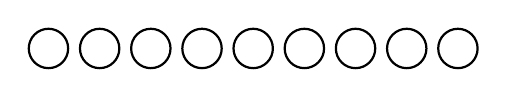
\begin{tikzpicture}
            \filldraw[fill=white, draw=black, thick] (1,1) circle (0.25cm);
            \filldraw[fill=white, draw=black, thick] (1.65,1) circle (0.25cm);
            \filldraw[fill=white, draw=black, thick] (2.3,1) circle (0.25cm);
            \filldraw[fill=white, draw=black, thick] (2.95,1) circle (0.25cm);
            \filldraw[fill=white, draw=black, thick] (3.6,1) circle (0.25cm);
            \filldraw[fill=white, draw=black, thick] (4.25,1) circle (0.25cm);
            \filldraw[fill=white, draw=black, thick] (4.9,1) circle (0.25cm);
            \filldraw[fill=white, draw=black, thick] (5.55,1) circle (0.25cm);
            \filldraw[fill=white, draw=black, thick] (6.2,1) circle (0.25cm);
        \end{tikzpicture} \\
        \scriptsize\normalfont\bfseries je Wunde AT, PA, FK, GE, INI - 2, GS - 1
    \end{dsaSheetBox}
}

\newcommand{\dsaTSHeading}[1]{\centering\normalfont\bfseries\scriptsize #1}

\newcommand{\LebensenergieAusdauerEtc}[2]{
    \begin{center}%
        \LARGE \shadowtext{Lebensenergie, Ausdauer, etc.}%
    \end{center}%
    \vspace{-12pt}

    \begin{dsaSheetBox}
        \tiny
        \begin{tabular}{p{3cm}|p{1cm}|p{1cm}|p{1cm}|p{1cm}|p{11.1cm}}
            & \dsaTSHeading{max.} & \dsaTSHeading{1/2} & \dsaTSHeading{1/3} & \dsaTSHeading{1/4} & \normalfont\bfseries\scriptsize\hspace{2pt} aktuell \\ \Xhline{2\arrayrulewidth}
            \footnotesize Lebensenergie & \textField[\ui{align={centered}}\textSize{9}\Ff{\FfReadOnly}]{LE-akt}{1cm}{10pt} & \mediumtext{LEdiv2}{1cm} & \mediumtext{LEdiv3}{1cm} & \mediumtext{LEdiv4}{1cm} & \\ \hline
            \footnotesize Ausdauer & \textField[\ui{align={centered}}\textSize{9}\Ff{\FfReadOnly}]{AU-akt}{1cm}{10pt} & \mediumtext{AUdiv2}{1cm} & \mediumtext{AUdiv3}{1cm} & \mediumtext{AUdiv4}{1cm} & \\ \hline
            \ifthenelse{\equal{#1}{1}}{
                \footnotesize Karmaenergie & \textField[\ui{align={centered}}\textSize{9}\Ff{\FfReadOnly}]{KE-akt}{1cm}{11.5pt} & \multicolumn{4}{l}{} \\ \hline
            }{}
            \ifthenelse{\equal{#2}{1}}{
                \footnotesize Astralenergie & \textField[\ui{align={centered}}\textSize{9}\Ff{\FfReadOnly}]{AE-akt}{1cm}{11.5pt} & \multicolumn{4}{l}{} \\ \hline
            }{}
        \end{tabular}

    \end{dsaSheetBox}
}

\Nahkampfwaffen{4}{4}

\Fernkampfwaffen{3}{3}

\begin{minipage}{12.6cm}
	\Waffenlos{4}
	\SchildParierwaffen{2}
	
	\vspace{4pt}
	\begin{minipage}{6cm}
		\Ruestung{6}
	\end{minipage}
	\begin{minipage}{6.5cm}
		\Ausweichen

		\vspace{-2pt}
		\Wunden
	\end{minipage}
\end{minipage}
\begin{minipage}{\textwidth-12.6cm-\fboxsep}
\Trefferzonenbild
\end{minipage}

\vspace{-10pt}
\LebensenergieAusdauerEtc{1}{1}

\end{dsaCharacterSheet}


\end{document}